\documentclass[a4paper,12pt]{article}

% Подключение необходимых пакетов
\usepackage[left=30mm,right=10mm,top=2cm,bottom=2cm]{geometry} % Поля 
\usepackage{amsmath,amsthm,amssymb}
\usepackage{mathtext}
\usepackage[T1,T2A]{fontenc}
\usepackage[utf8]{inputenc}
\usepackage[english,russian]{babel}
\usepackage{graphicx}
\usepackage{tabularx} % Пакет для таблиц с автоматической шириной столбцов

\usepackage{setspace} % Межстрочные интервалы
\usepackage{indentfirst} % Отступ у первого абзаца
\usepackage{titlesec} % Настройка заголовков
\usepackage{csquotes} % Для цитат
\usepackage{hyperref} % Для гиперссылок
\usepackage{amsmath}
\usepackage{amssymb}
\usepackage{xypic}
\usepackage{tikz}

\usepackage{listings}
\lstset{inputencoding=utf8x, extendedchars=\true}

% Define a custom color
\definecolor{backcolour}{rgb}{0.95,0.95,0.92}
\definecolor{codegreen}{rgb}{0,0.6,0}

% Define a custom style
\lstdefinestyle{myStyle}{
	backgroundcolor=\color{backcolour},   
	commentstyle=\color{codegreen},
	basicstyle=\ttfamily\footnotesize,
	breakatwhitespace=false,         
	breaklines=true,                 
	keepspaces=true,                 
	numbers=left,       
	numbersep=5pt,                  
	showspaces=false,                
	showstringspaces=false,
	showtabs=false,                  
	tabsize=2,
	basicstyle=\footnotesize\ttfamily,
	keywordstyle=\bfseries\color{green!40!black},
	commentstyle=\itshape\color{purple!40!black},
	identifierstyle=\color{blue},
	backgroundcolor=\color{gray!10!white},
}

% Use \lstset to make myStyle the global default
\lstset{style=myStyle}


\usetikzlibrary{positioning}

% Форматирование заголовков разделов
\titleformat{\section}{\bfseries\fontsize{14pt}{14pt}\selectfont}{\thesection.}{1em}{}
\titlespacing{\section}{0pt}{6pt}{6pt}

% Настройка абзацев
\setlength{\parindent}{1.25cm} % Абзацный отступ
\setlength{\parskip}{6pt} % Интервал между абзацами

% Оформление цитат
\newenvironment{quoteformat}{\bfseries}{}

\begin{document}
	\begin{titlepage}
		\begin{center}
			% Шапка
			{\large \textbf{Министерство науки и высшего образования \\ Российской Федерации}}
			
			{\large\textbf{Федеральное государственное автономное образовательное учреждение высшего образования}}
			
			{\large \textbf{«Южно-Уральский государственный университет (НИУ)»}}
			
			{\large \textbf{Высшая школа электроники и компьютерных наук}}
			
			{\large \textbf{Кафедра системного программирования}\\[2cm]
			}
			% Тип работы
			\textbf{ОТЧЕТ}\\[0.2cm]
			о выполнении дополнительного практического задания №2\\[0.2cm]
			по дисциплине\\[0.2cm]
			«Структуры и алгоритмы обработки данных»\\[0.2cm]
			\textbf{Вариант 5}\\[3cm]
		\end{center}
		
		\begin{flushright}
			Проверил:\\[0.2cm]
			ст. преподаватель кафедры СП\\[0.2cm]
			\textbf{Петрова Л.Н.}\\[1cm]
						
			Выполнил:\\[0.2cm]
			Студент группы КЭз-391\\[0.2cm]
			\textbf{Галиулин Р.Р.}\\[0.2cm]
			
		\end{flushright}
		\vfill{}
		
		\begin{center}
			Челябинск \\ 2025
		\end{center}
	\end{titlepage}
	\newpage
	
	\tableofcontents
	
	\setcounter{page}{2}
	\newpage
	%\maketitle
	\section{Описание задачи}
	\textbf{Задание: Двоичные (бинарные) деревья}
	
	Используя рекурсивную функцию, напишите программу, которая вычисляет среднее арифметическое всех элементов непустого бинарного дерева
	
	\textbf{Входные данные}
	
	Данные вводимые пользователем отсутствуют.
	
	\begin{itemize}
		\item Количество узлов (листьев) бинарного дерева - определяется автоматически с помощью генератора псевдослучайный чисел на основе времени в диапазоне [2..30]
		\item Значения узлов (листьев) бинарного дерева - определяется автоматически с помощью генератора псевдослучайный чисел на основе времени в диапазоне [0..99]
	\end{itemize} 
	
	\textbf{Выходные данные}
	
	\begin{itemize}
		\item Среднее арифметическое до удаления - вещественное число
		\item Изображение дерева с помощью псевдографики, до удаления
		\item Среднее арифметическое после удаления - вещественное число
		\item Изображение дерева с помощью псевдографики, после удаления
		
	\end{itemize} 

	\textit{Все данные выводятся с помощью стандартного потока вывода}	
	
	При разработке программы применялась следующая логика обработки удаления элемента бинарного дерева.
	
	При удалении узла из бинарного дерева возможны три случая:
	
	\begin{itemize}
		\item Удаление листового узла (у узла нет потомков) \newline
	Просто удаляем узел, никаких дополнительных действий не требуется.
		\item Удаление узла с одним потомком \newline
	Заменяем удаляемый узел его единственным потомком. \newline
	Родитель удаляемого узла начинает ссылаться на этого потомка.
			\item 	Удаление узла с двумя потомками \newline
	Находим наименьший узел в правом поддереве (или наибольший в левом). \newline
	Копируем его значение в удаляемый узел. \newline
	Удаляем этот найденный узел (он гарантированно имеет не более одного потомка, поэтому его удаление попадает под один из первых двух случаев). \newline
	\end{itemize}
	Таким образом, структура дерева изменяется, но остается корректной. 

	
	
	\newpage	
	\section{Листинг программы}
	Язык программирования: C++ 14. Среда разработки: Ubuntu 24.10, gcc 14.2.0, nvim
	\lstinputlisting[caption=Задание: Двоичные (бинарные) деревья,label={lst:listing-cpp}, language=C++, firstline=1]{app9.cpp}
	

	\newpage
	\section{Контрольные тесты}
	
	\begin{center}
		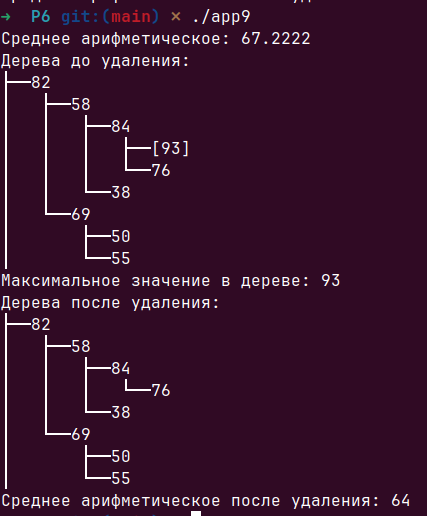
\includegraphics[width=0.7\linewidth]{fig/fig1}
	\end{center}
	
	\begin{center}
		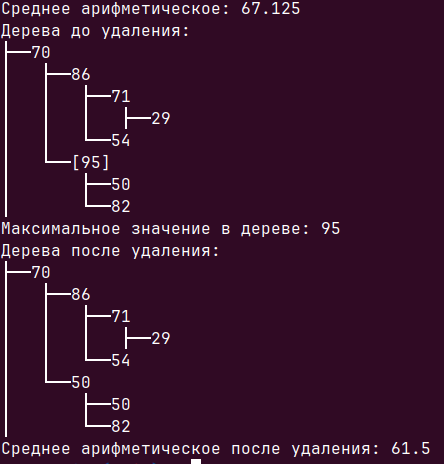
\includegraphics[width=0.7\linewidth]{fig/fig2}
	\end{center}
	

\renewcommand{\arraystretch}{1.5} % Увеличиваем высоту строк
\subsection{Задание №1: Двух связанный список}
\begin{table}[ht]
	
	\centering
	\begin{tabularx}{\textwidth}{|X|X|}
		\hline
		\textbf{Исходные данные} & \textbf{Результат} \\ \hline
		10 \newline 43 45 86 11 94 29 75 99 41 12 & 
		Исходный список: \newline 43 45 86 11 94 29 75 [99] 41 12 \newline
		Список после удаления максимального элемента: \newline 43 45 86 11 94 29 75 41 12 \\ \hline
		
		5 \newline 5 5 9 2 10 & 
		Исходный список: \newline 5 5 9 2 [10] \newline
		Список после удаления максимального элемента: \newline 5 5 9 2 \\ \hline
		
	\end{tabularx}
	\caption{Таблица с результатами контрольных тестов Задания №1}
\end{table}
	
\end{document}